\documentclass[10pt,a4paper,openany]{article}
\usepackage[latin1]{inputenc}
\usepackage{amsmath}
\usepackage{amsfonts}
\usepackage{amssymb}
\usepackage{graphicx}
\usepackage{listings}
\usepackage{color}
\usepackage[left=2cm,right=2cm,top=3cm,bottom=2cm]{geometry}
\usepackage[numbers,sort&compress]{natbib}
\usepackage[english]{babel}
\usepackage{url}
\usepackage{caption}

\setlength{\parindent}{0pt}

\definecolor{mygreen}{rgb}{0,0.6,0}
\definecolor{mygray}{rgb}{0.5,0.5,0.5}
\definecolor{mymauve}{rgb}{0.58,0,0.82}

\lstset{ 
	backgroundcolor=\color{white},   % choose the background color; you must add \usepackage{color} or \usepackage{xcolor}; should come as last argument
	basicstyle=\footnotesize,        % the size of the fonts that are used for the code
	breakatwhitespace=false,         % sets if automatic breaks should only happen at whitespace
	breaklines=true,                 % sets automatic line breaking
	captionpos=b,                    % sets the caption-position to bottom
	commentstyle=\color{mygreen},    % comment style
	deletekeywords={...},            % if you want to delete keywords from the given language
	escapeinside={\%*}{*)},          % if you want to add LaTeX within your code
	extendedchars=true,              % lets you use non-ASCII characters; for 8-bits encodings only, does not work with UTF-8
	firstnumber=01,                	 % start line enumeration with line 1000
	frame=single,	                 % adds a frame around the code
	keepspaces=true,                 % keeps spaces in text, useful for keeping indentation of code (possibly needs columns=flexible)
	keywordstyle=\color{blue},       % keyword style
	language=Python,                 % the language of the code
	morekeywords={*,...},            % if you want to add more keywords to the set
	numbers=left,                    % where to put the line-numbers; possible values are (none, left, right)
	numbersep=5pt,                   % how far the line-numbers are from the code
	numberstyle=\tiny\color{mygray}, % the style that is used for the line-numbers
	rulecolor=\color{black},         % if not set, the frame-color may be changed on line-breaks within not-black text (e.g. comments (green here))
	showspaces=false,                % show spaces everywhere adding particular underscores; it overrides 'showstringspaces'
	showstringspaces=false,          % underline spaces within strings only
	showtabs=false,                  % show tabs within strings adding particular underscores
	stepnumber=1,                    % the step between two line-numbers. If it's 1, each line will be numbered
	stringstyle=\color{mymauve},     % string literal style
	tabsize=2,	                     % sets default tabsize to 2 spaces
	title=\lstname                   % show the filename of files included with \lstinputlisting; also try caption instead of title
}

\author{5273}
\title{Homework Assignment 2: Network Flows}
\date{}

\begin{document}
	
\maketitle
	
	\section*{Circular Layout}
	As the name suggest this layout positions nodes in a circle \citep{networkx}. According to \citep{tsay2010hierarchically} although this algorithm can appear trivial, it is widely used to visualize complexes and pathways. The algorithm attempts to minimize the number of overlapping nodes and edges, this way interactions among nodes are easier to understand and locate.  It allows to highlight the node or nodes with the highest degree, moreover it evidences potencially interesting sub-networks as inner circles in the network \citep{agapito2013visualization}.
	
	\lstinputlisting[language=Python]{graph02ucg.py}
	
	\begin{center}
		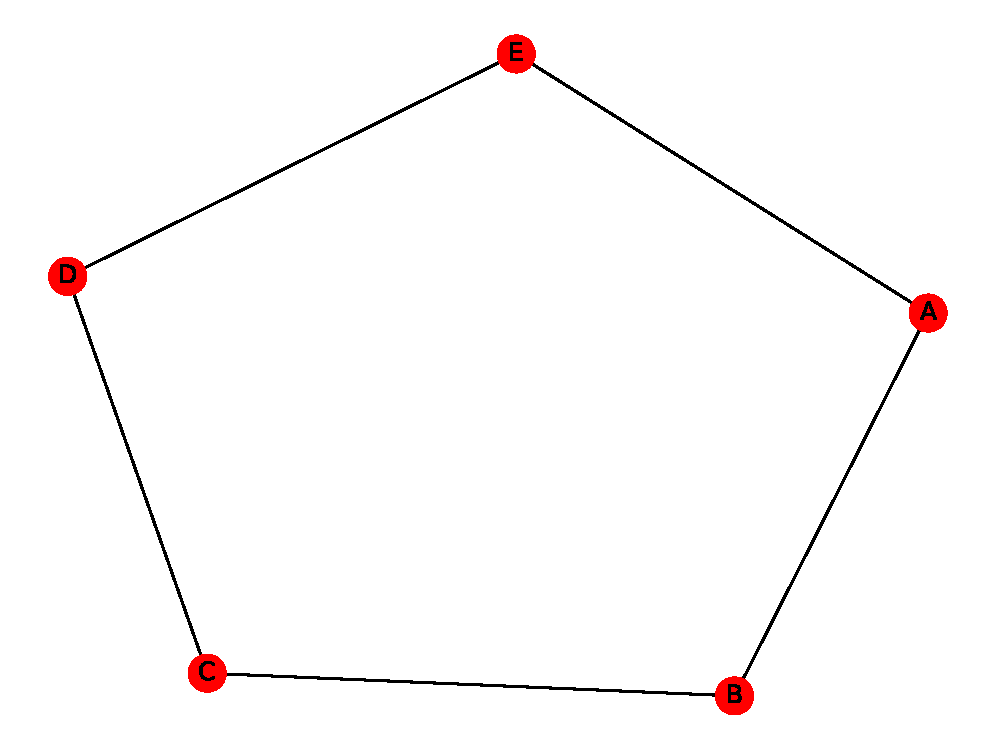
\includegraphics[scale=0.8]{Graph02}
		\captionof{figure}{Circular layout}
	\end{center}
	
\newpage
	
	\section*{Random Layout}
	This algorithm positions nodes by choosing coordinates uniformly at random on the interval [0.0, 1.0) where the nodes are generated \citep{networkx}. 
	The advantage of this kind of layout lays in the  very  fast drawing on  the  network  graph.  However it carries  the  disadvantage  of  the  difficulty in grasping the position of nodes \citep{mouri2016visualization}.
	
	\lstinputlisting[language=Python]{graph06drg.py}
	
	\begin{center}
		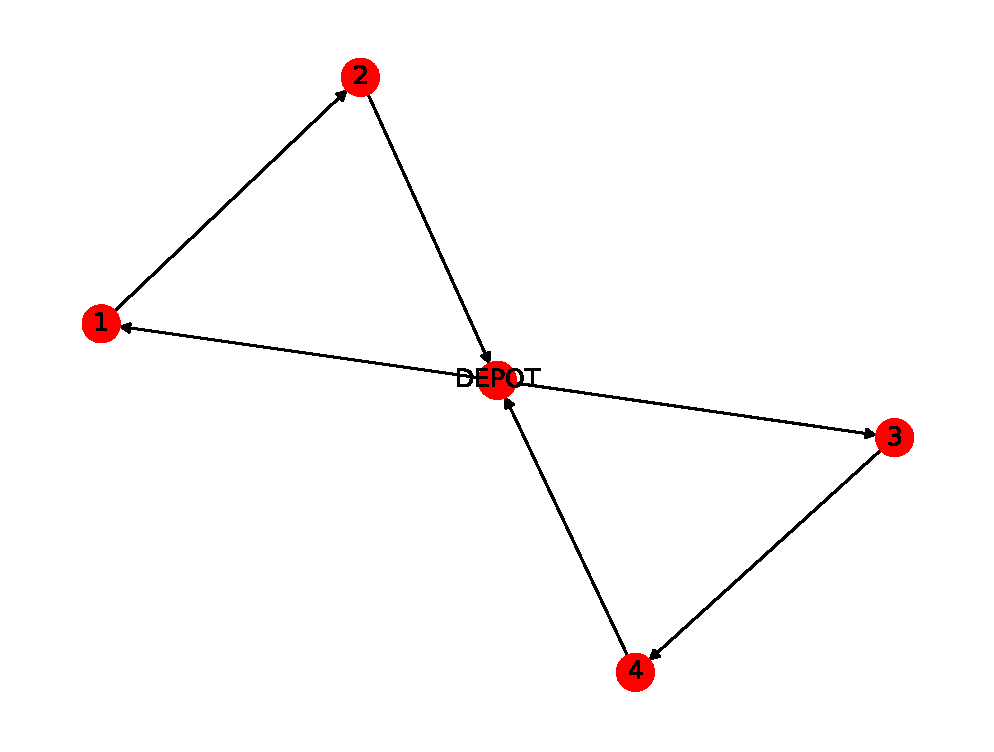
\includegraphics[scale=0.8]{Graph06}
		\captionof{figure}{Random layout}
	\end{center}

\newpage
	
	\section*{Bipartite Layout}
	This layout positions nodes in two straight lines \citep{networkx}. This particular class only allows the connection between two nodes in different sets \citep{easley2010networks}. Nodes from set X are only connected with nodes from set Y, not with other nodes from X, and vice versa \citep{seminar2014}.
	
	\lstinputlisting[language=Python]{graph11dcm.py}
	
	\begin{center}
		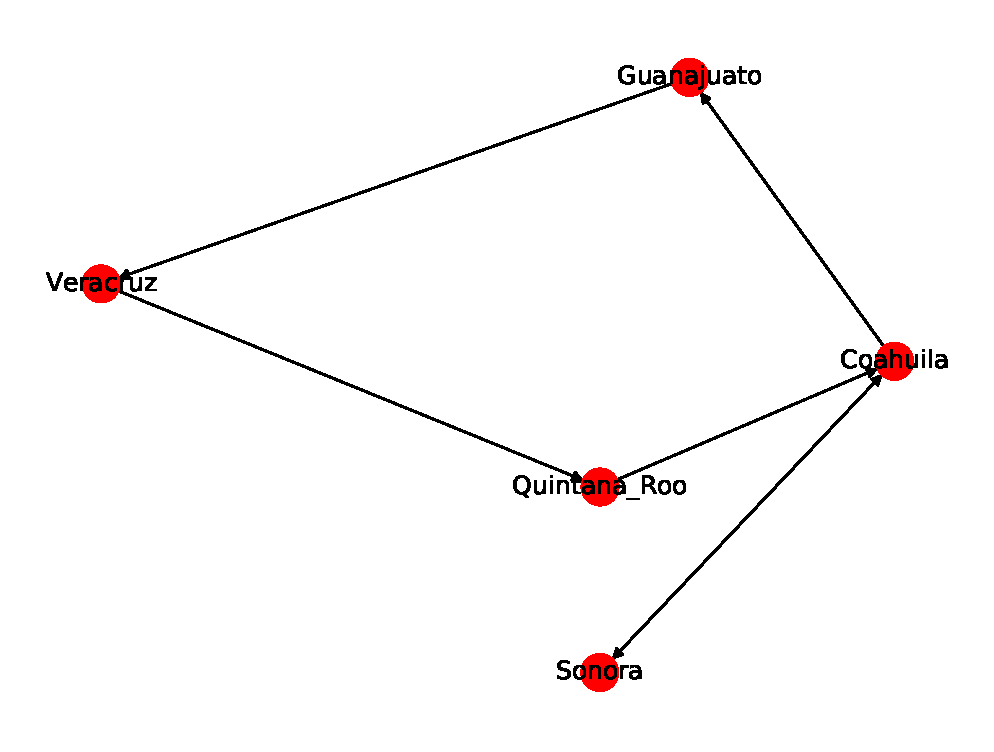
\includegraphics[scale=0.8]{Graph11}
		\captionof{figure}{Bipartite layout}
	\end{center}
	
\newpage	
	
	\section*{Kamada-Kawai Layout}
	Is an algorithm for drawing undirected graphs and weighted graphs and is based on the concept of theoretic distance between nodes \citep{kamada1989algorithm}. In this algorithm the forces between the nodes can be determined by the lengths of shortest paths between each couple of nodes \citep{networkx}. The classical Kamada-Kawai algorithm does not scale well when it is used in networks with large numbers of nodes \citep{DBLP:journals/corr/CheongS15}.
	
	This layout will be represented by an undirected reflexive graph and a directed acyclic multigraph.
	
		\subsection*{Undirected reflexive graph}
		\lstinputlisting[language=Python]{graph03urg.py}
	
		\begin{center}
			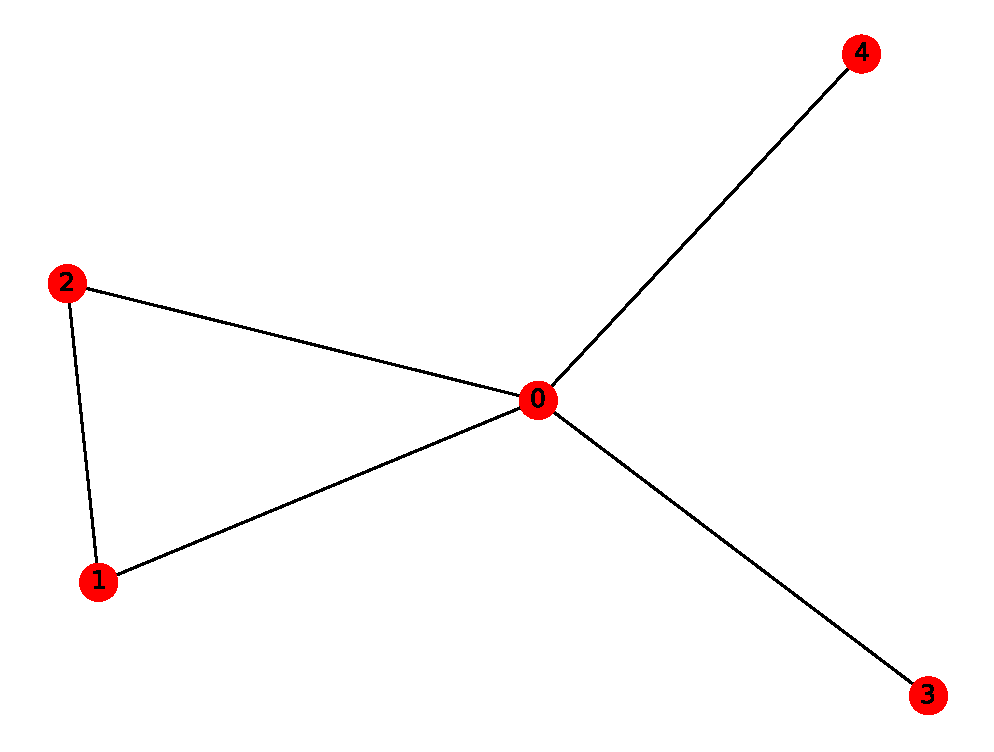
\includegraphics[scale=0.8]{Graph03}
			\captionof{figure}{Kamada-Kawai layout for the undirected reflexive graph}
		\end{center}
	
	\newpage
	
		\subsection*{Directed acyclic multigraph}
		\lstinputlisting[language=Python]{graph10dam.py}

		\begin{center}
			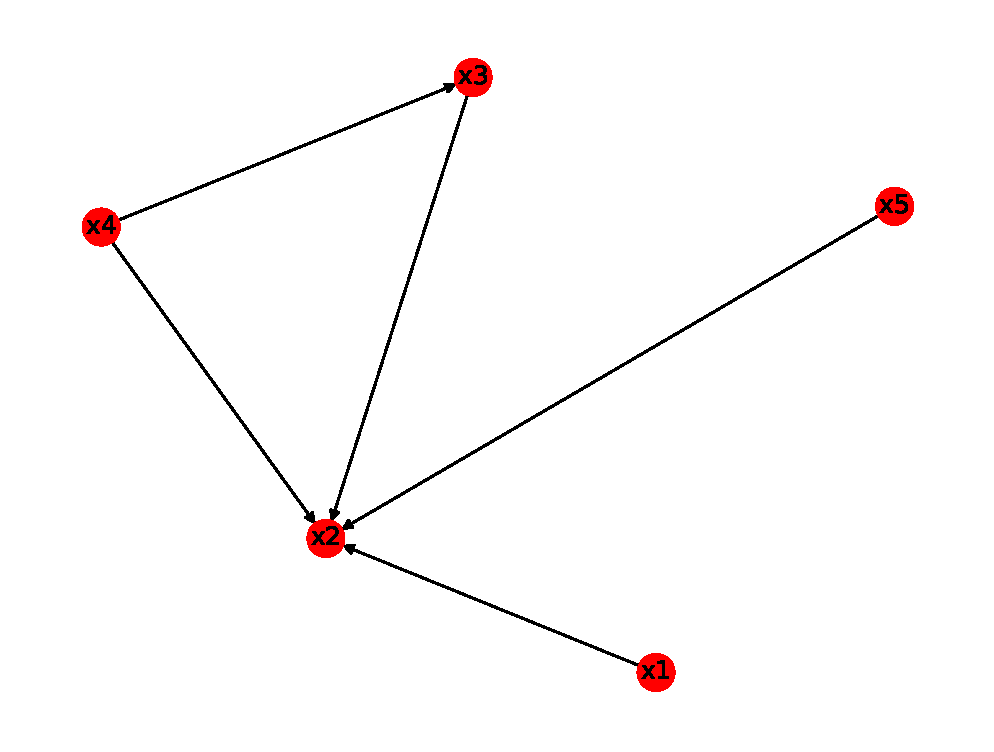
\includegraphics[scale=0.8]{Graph10}
			\captionof{figure}{Kamada-Kawai layout for the directed acyclic multigraph}
		\end{center}
	
	
\newpage
	
	\section*{Shell Layout}
	This layout positions nodes in concentric circles \citep{networkx}. It is also known as concentric layout in \citep{cherven2015mastering}, where it is said that this arrangement in a series of concentric circles is based on the distance from the central node. Thus, nodes with direct connections are arranged in the first circle, then the nodes located at a distance of two nodes away from the center follows in this arrengement and so on, until the graph is completed. The main advantage of this layout is that viewers are able to see network structures easier and to navigate them noticing the closeness of relationships to a single node to each other.
	
	This layout will be represented by a directed cyclic graph and a directed reflexive multigraph.
	
		\subsection*{Directed cyclic graph}
		
		\lstinputlisting[language=Python]{graph05dcg.py}
	
		\begin{center}
			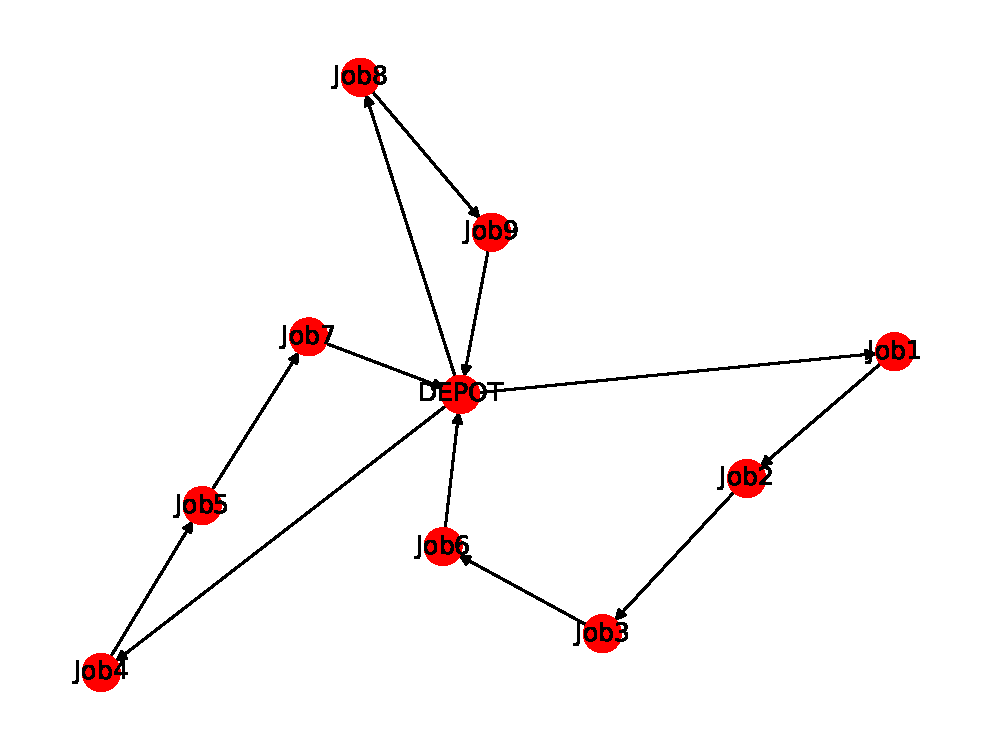
\includegraphics[scale=0.8]{Graph05}
			\captionof{figure}{Shell layout for the directed cyclic graph}
		\end{center}
	
	\newpage
	
		\subsection*{Directed reflexive multigraph}
		
		\lstinputlisting[language=Python]{graph12drm.py}
		
		\begin{center}
			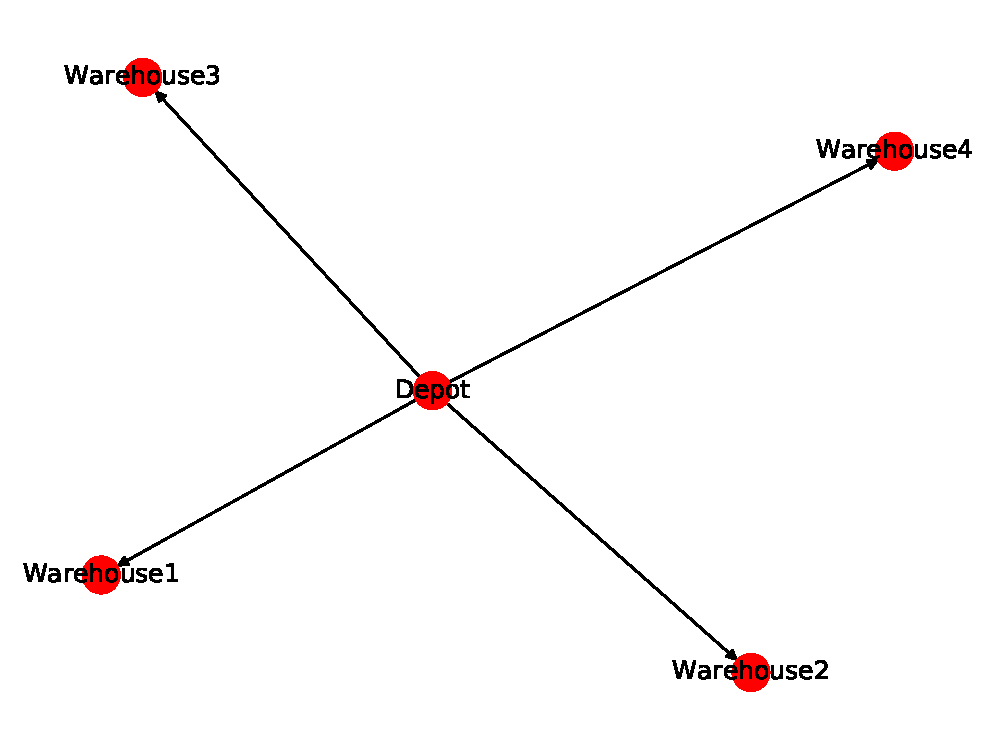
\includegraphics[scale=0.8]{Graph12}
			\captionof{figure}{Shell layout for the directed cyclic graph}
		\end{center}
	
\newpage
	
	\section*{Fruchterman-Reingold Layout}
	This algorithm attempts to distribute vertices evenly, make edge lengths uniform, and reflect symmetry \citep{fruchterman1991graph}. Is best for fewer than thirty
	nodes and does not require parameters to be optimised \citep{gibson2013survey}.
	This layout will be represented by an undirected acyclic multigraph and a directed acyclic graph.
	
		\subsection*{Undirected acyclic multigraph}
	
		\lstinputlisting[language=Python]{graph07uam.py}
	
		\begin{center}
			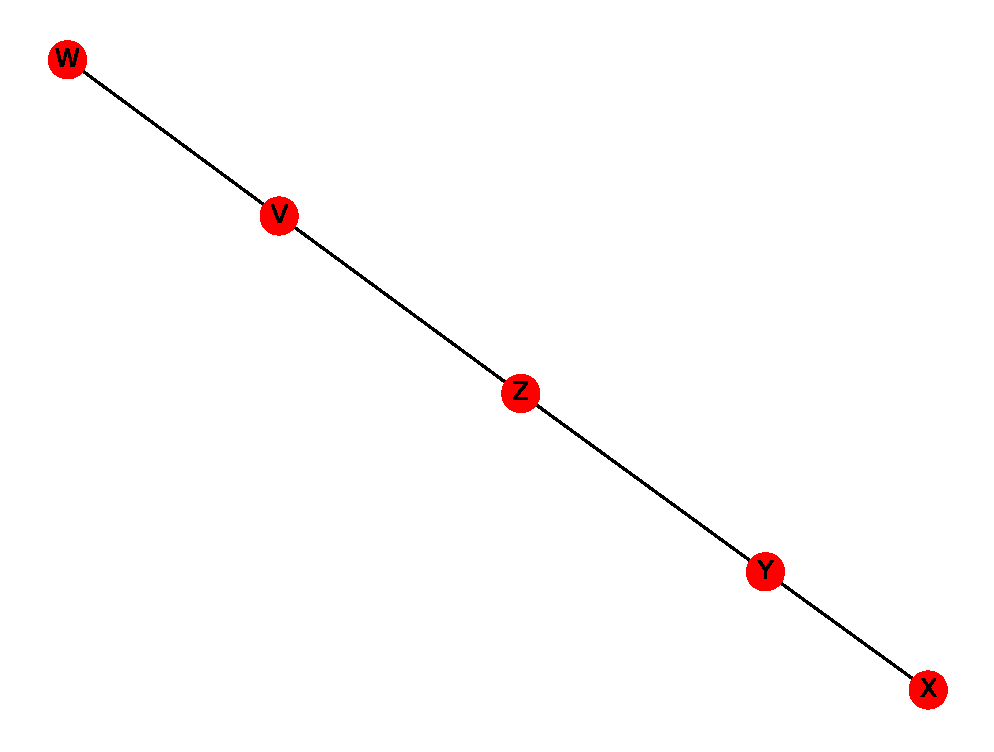
\includegraphics[scale=0.8]{Graph07}
			\captionof{figure}{Fruchterman-Reingold layout for the undirected acyclic multigraph}
		\end{center}
	
		\newpage

		\subsection*{Directed acyclic graph}
		
		\lstinputlisting[language=Python]{graph04dag.py}
		
		\begin{center}
			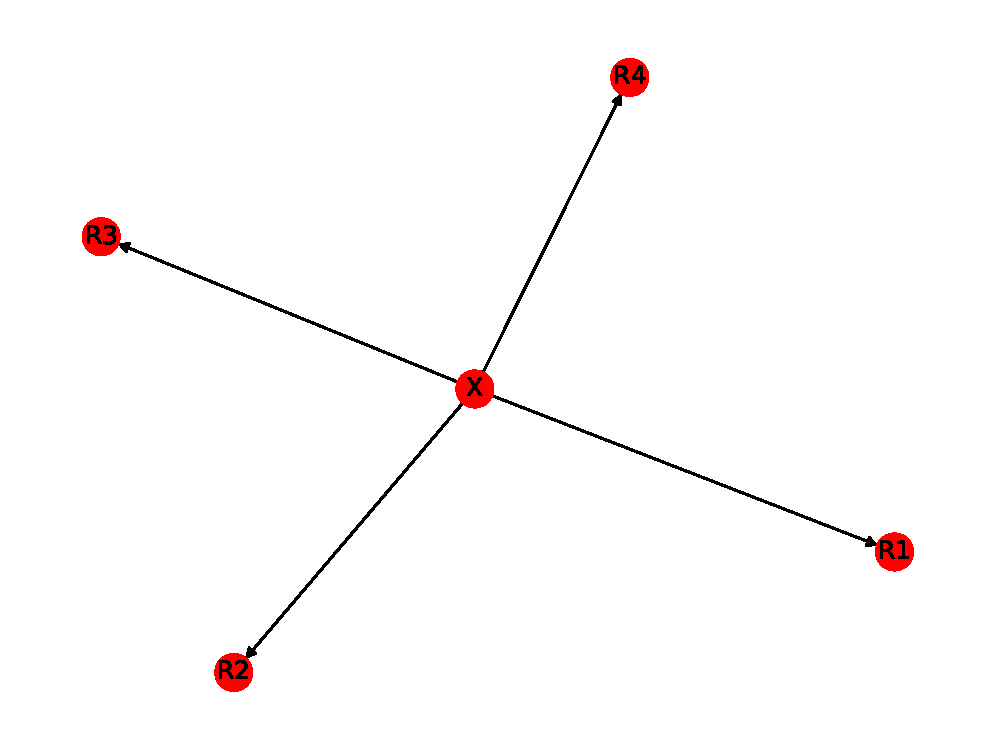
\includegraphics[scale=0.8]{Graph04}
			\captionof{figure}{Fruchterman-Reingold layout for the directed acyclic graph}
		\end{center}

\newpage

	\section*{Spring Layout}
	This layout positions nodes using the algorithm of Fruchterman-Reingold \citep{networkx}. The algorithm first places the vertices in some initial layout and then it moves the rings in which the system reach a minimal energy due to the spring forces. With this layout we should obtain a display as much symmetry as possible \citep{DBLP:journals/corr/abs-1201-3011}.
	
	\lstinputlisting[language=Python]{graph08ucm.py}
	
	\begin{center}
		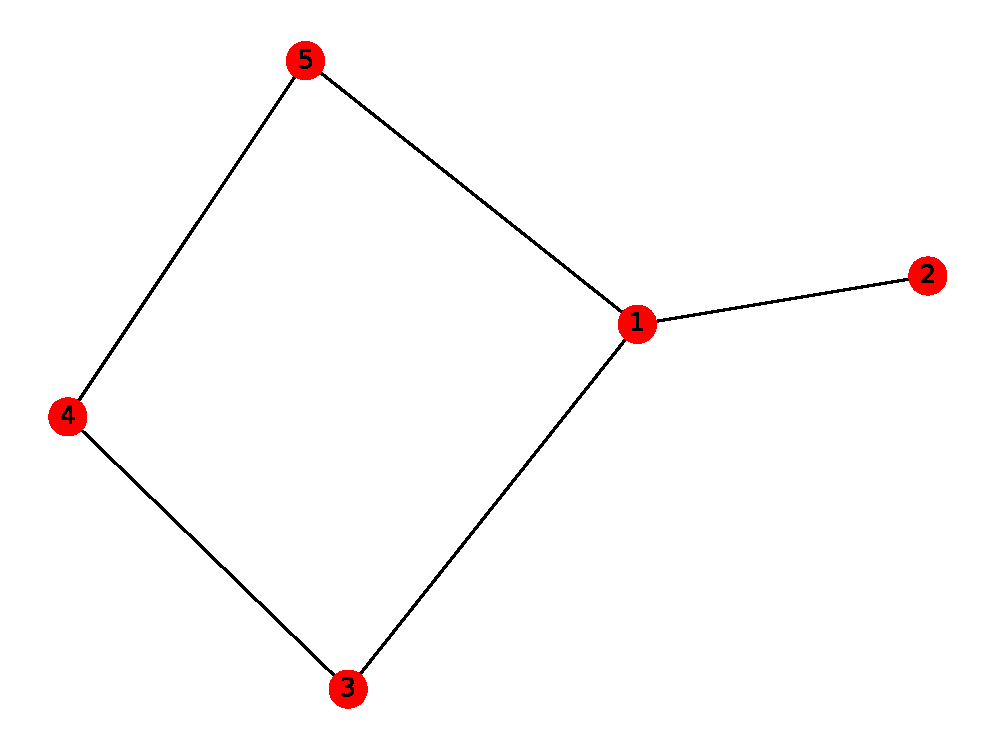
\includegraphics[scale=0.8]{Graph08}
		\captionof{figure}{Spring layout}
	\end{center}
	
\newpage
	
	\section*{Spectral Layout}
	This approach has the advantage of computing optimal layouts (according to some requirements) and rapid computation time. It provides an exact solution to the layout problem, whereas other formulations end in an NP-hard problem with approximated solutions \citep{koren2003spectral}. To construct the layout it uses eigenvectors of the adjacency matrix of the graph and of the Laplacian spectrum associated with the graph \citep{koren2003spectral}. While we use this layout in Python using NetworkX, positioning the nodes, directed graphs will be considered as unidrected graphs \citep{networkx}.
	
	\lstinputlisting[language=Python]{graph09urm.py}
	
	\begin{center}
		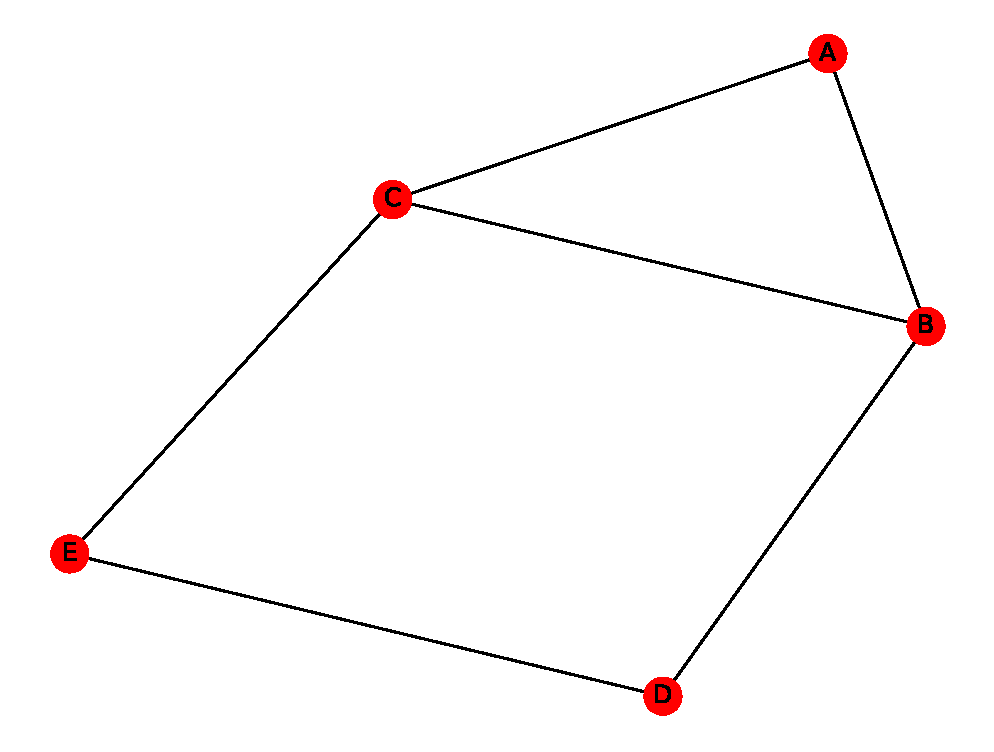
\includegraphics[scale=0.8]{Graph09}
		\captionof{figure}{Spectral layout}
	\end{center}
	
\newpage

	\section*{Force Atlas 2 Layout}
	Force Atlas 2 is a very fast layout algorithm for force-directed graphs. It's used to spatialize a weighted undirected graph in 2D (Edge weight defines the strength of the connection). The implementation is based on \citep{jacomy2014forceatlas2}. Its really quick compared to the fruchterman reingold algorithm (spring layout) of networkx and scales well to high number of nodes.
	
	\lstinputlisting[language=Python]{graph01uag.py}
	
	\begin{center}
		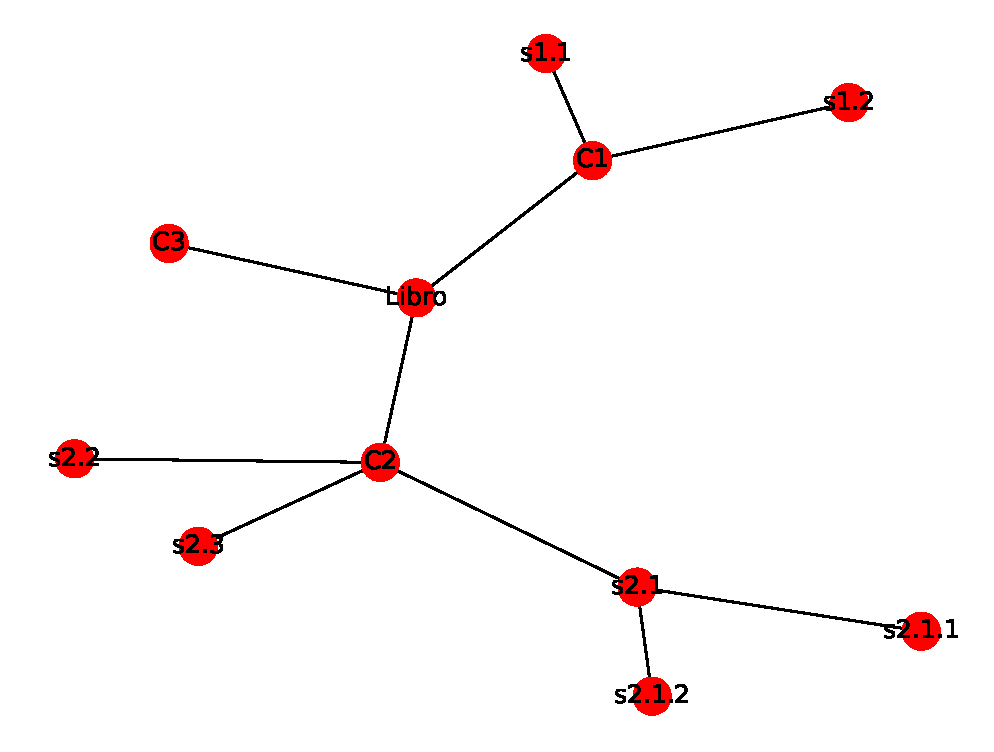
\includegraphics[scale=0.8]{Graph01}
		\captionof{figure}{Force Atlas 2 layout}
	\end{center}
	

	\bibliography{tarea2}
	\bibliographystyle{plainnat}
	
\end{document}